\emph{In problems 1--4, write an objective function for the given situation in terms of the variables defined.}
\begin{enumerate}
\item A fence company sells wooden and metal fences.  Let $x$ represent the number of wooden fences they sell and let $y$ represent the number of metal fences.  They make a profit of \$320 for each wooden fence and \$280 for each metal fence. \answer{$p = 320x + 280y$}

\item You are placing mulch in your yard, and you find that pine chips cost \$2 per bag, while oak chips cost \$4 per bag.  You want to minimize total cost.  Let $x$ be the number of bags of pine chips and $y$ be the number of bags of oak chips. \answer{$c = 2x + 4y$}

\item An auto repair shop offers tire rotations and oil changes.  They make a profit of \$25 on each oil change and a profit of \$18 on each tire rotation.  Let $x$ be the number of oil changes and $y$ be the number of tire rotations. \answer{$p = 25x + 18y$}

\item Taking a pill of Medicine A gives you 6 mg of an undesired substance, and Medicine B gives you 8 mg of the undesired substance (you want to minimize the amount of this substance).  Let $x$ be the number of A pills you take and $y$ be the number of B pills you take.
\answer{$u = 6x + 8y$}
\end{enumerate}

\emph{In problems 5--8, write an inequality to represent each constraint given.}
\begin{enumerate}
\setcounter{enumi}{4}

\item Manufacturing one chair ($x$) requires 6 ft of aluminum tube, and manufacturing one table ($y$) requires 12 ft of aluminum tube.  There are 500 ft of aluminum tube available. \answer{$6x + 12y \leq 500$}

\item Each oil change ($x$) takes 20 minutes and each tire rotation ($y$) takes 15 minutes.  There are a total of 2400 minutes available. \answer{$20x + 15y \leq 2400$}

\item You must take at least 3 pills of Medicine A ($x$) and at least 2 pills of Medicine B ($y$). \answer{$x \geq 3; y \geq 2$}

\item Mowing a large yard ($x$) uses 0.25 gallons of gasoline, and mowing a small yard ($y$) uses 0.1 gallons of gasoline.  There are 5 gallons of gasoline available. \answer{$0.25x + 0.1y \leq 5$}
\end{enumerate}
\vfill
\pagebreak

\emph{In problems 9--12, graph each feasible region and list the corner points.}
\begin{enumerate}
\setcounter{enumi}{8}

\item Feasible region:
\begin{align*}
2x+4y &\leq 20\\
4x+2y &\leq 16\\
x &\geq 0\\
y &\geq 0
\end{align*}
\begin{center}
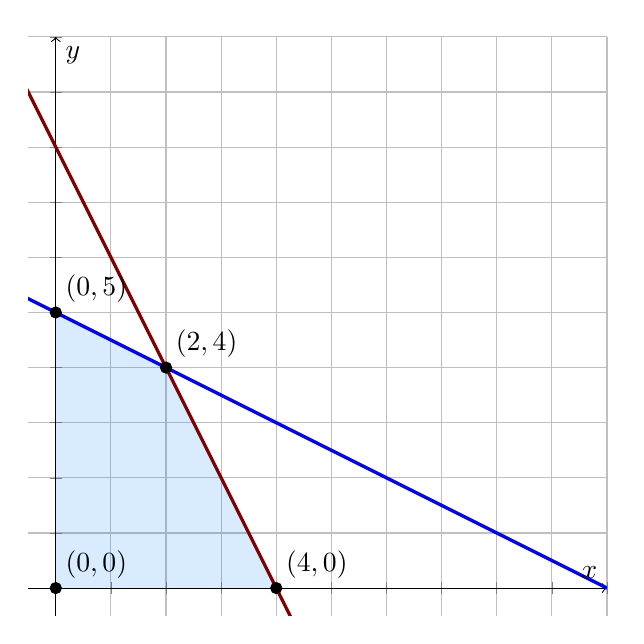
\begin{tikzpicture}
\begin{axis}[
    xmin=-0.5, xmax=10,
    ymin=-0.5, ymax=10,
    axis lines=center,
    axis on top=false,
    domain=0:1,
    x=0.7cm,
    y=0.7cm,
    xtick={0,1,...,10},
    xticklabels={},
    ytick={0,1,...,10},
    yticklabels={},
    axis lines=middle,
    axis line style={->},
    xlabel={$x$},
    ylabel={$y$},
    grid=major
    ]
    \addplot [thick,color=blue,fill=blue!50!cyan, 
                    fill opacity=0.15,draw opacity=0]coordinates {
            (0,0)
            (0,5)
            (2,4)
            (4,0)  };
    \addplot [very thick,blue,domain=-10:10] {-x/2+5};
    \addplot [very thick,red!50!black,domain=-10:10] {-2*x+8};
	%\addplot [very thick,red!50!black] coordinates{(-3,-5)(-3,5)};
	
	\addplot [only marks,color=black] table {
	0 5
	0 0
	4 0
	2 4
	};  
	\node[above right] (A) at (axis cs:2,4) {$(2,4)$};
	\node[above right] (B) at (axis cs:0,5) {$(0,5)$};
	\node[above right] (C) at (axis cs:4,0) {$(4,0)$};
	\node[above right] (D) at (axis cs:0,0) {$(0,0)$};
\end{axis}
\end{tikzpicture}
\end{center}

\item Feasible region:
\begin{align*}
20x+40y &\leq 160\\
18x+9y &\leq 90\\
x &\geq 0\\
y &\geq 0
\end{align*}
\begin{center}
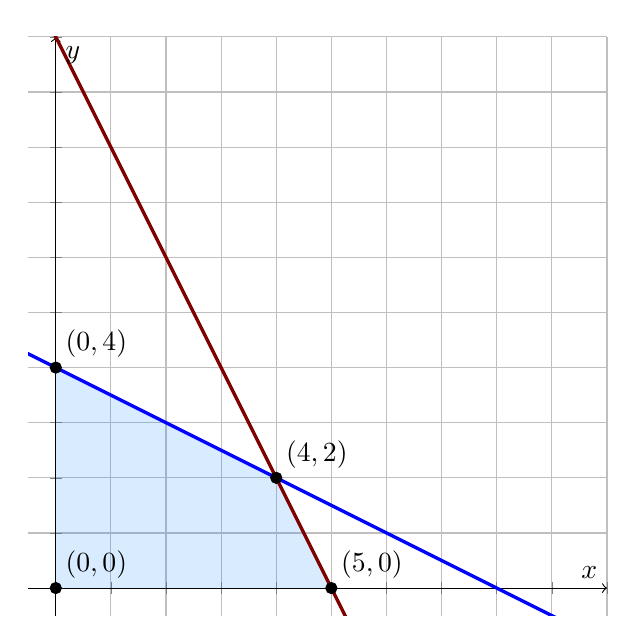
\begin{tikzpicture}
\begin{axis}[
    xmin=-0.5, xmax=10,
    ymin=-0.5, ymax=10,
    axis lines=center,
    axis on top=false,
    domain=0:1,
    x=0.7cm,
    y=0.7cm,
    xtick={0,1,...,10},
    xticklabels={},
    ytick={0,1,...,10},
    yticklabels={},
    axis lines=middle,
    axis line style={->},
    xlabel={$x$},
    ylabel={$y$},
    grid=major
    ]
    \addplot [thick,color=blue,fill=blue!50!cyan, 
                    fill opacity=0.15,draw opacity=0]coordinates {
            (0,0)
            (0,4)
            (4,2)
            (5,0)  };
    \addplot [very thick,blue,domain=-10:10] {-x/2+4};
    \addplot [very thick,red!50!black,domain=-10:10] {-2*x+10};
	%\addplot [very thick,red!50!black] coordinates{(-3,-5)(-3,5)};
	
	\addplot [only marks,color=black] table {
	0 4
	0 0
	5 0
	4 2
	};  
	\node[above right] (A) at (axis cs:4,2) {$(4,2)$};
	\node[above right] (B) at (axis cs:0,4) {$(0,4)$};
	\node[above right] (C) at (axis cs:5,0) {$(5,0)$};
	\node[above right] (D) at (axis cs:0,0) {$(0,0)$};
\end{axis}
\end{tikzpicture}
\end{center}

\item Feasible region:
\begin{align*}
2x+y &\leq 8\\
x+3y &\leq 6\\
x &\geq 0\\
y &\geq 0
\end{align*}
\begin{center}
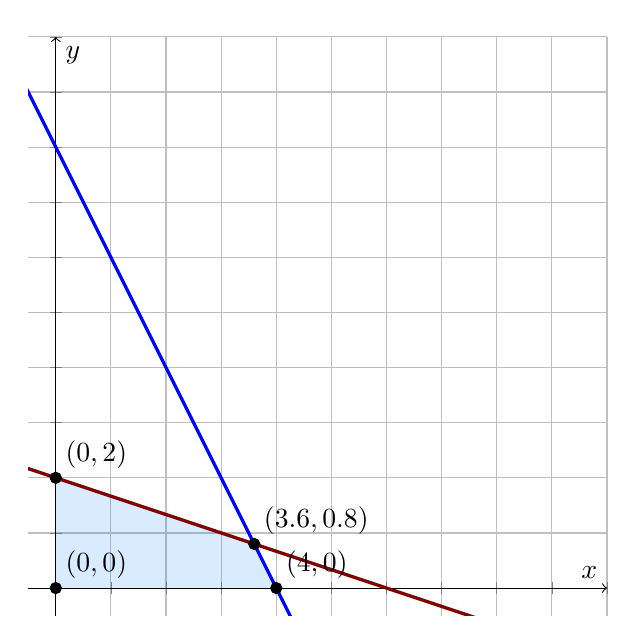
\begin{tikzpicture}
\begin{axis}[
    xmin=-0.5, xmax=10,
    ymin=-0.5, ymax=10,
    axis lines=center,
    axis on top=false,
    domain=0:1,
    x=0.7cm,
    y=0.7cm,
    xtick={0,1,...,10},
    xticklabels={},
    ytick={0,1,...,10},
    yticklabels={},
    axis lines=middle,
    axis line style={->},
    xlabel={$x$},
    ylabel={$y$},
    grid=major
    ]
    \addplot [thick,color=blue,fill=blue!50!cyan, 
                    fill opacity=0.15,draw opacity=0]coordinates {
            (0,0)
            (0,2)
            (18/5,4/5)
            (4,0)  };
    \addplot [very thick,blue,domain=-10:10] {-2*x+8};
    \addplot [very thick,red!50!black,domain=-10:10] {-x/3+2};
	%\addplot [very thick,red!50!black] coordinates{(-3,-5)(-3,5)};
	
	\addplot [only marks,color=black] table {
	0 2
	0 0
	4 0
	3.6 0.8
	};  
	\node[above right] (A) at (axis cs:3.6,0.8) {$(3.6,0.8)$};
	\node[above right] (B) at (axis cs:0,2) {$(0,2)$};
	\node[above right] (C) at (axis cs:4,0) {$(4,0)$};
	\node[above right] (D) at (axis cs:0,0) {$(0,0)$};
\end{axis}
\end{tikzpicture}
\end{center}

\item Feasible region:
\begin{align*}
15x+5y &\leq 75\\
9x+9y &\leq 81\\
x &\geq 0\\
y &\geq 0
\end{align*}
\begin{center}
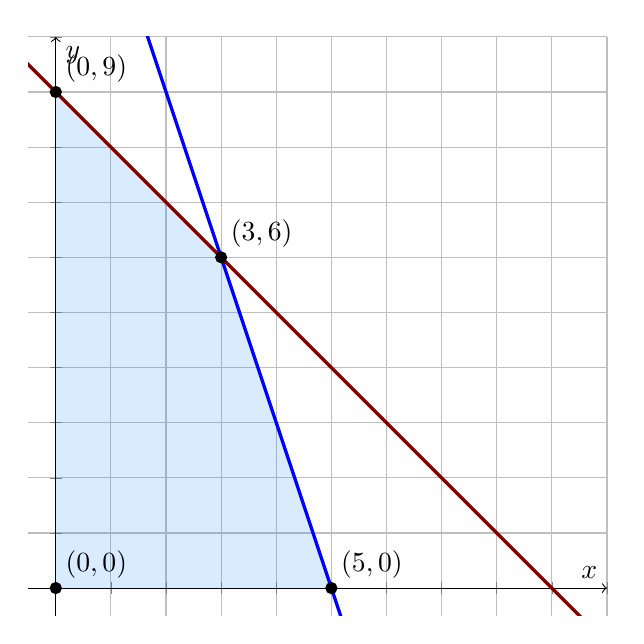
\begin{tikzpicture}
\begin{axis}[
    xmin=-0.5, xmax=10,
    ymin=-0.5, ymax=10,
    axis lines=center,
    axis on top=false,
    domain=0:1,
    x=0.7cm,
    y=0.7cm,
    xtick={0,1,...,10},
    xticklabels={},
    ytick={0,1,...,10},
    yticklabels={},
    axis lines=middle,
    axis line style={->},
    xlabel={$x$},
    ylabel={$y$},
    grid=major
    ]
    \addplot [thick,color=blue,fill=blue!50!cyan, 
                    fill opacity=0.15,draw opacity=0]coordinates {
            (0,0)
            (0,9)
            (3,6)
            (5,0)  };
    \addplot [very thick,blue,domain=-10:10] {-3*x+15};
    \addplot [very thick,red!50!black,domain=-10:10] {-x+9};
	%\addplot [very thick,red!50!black] coordinates{(-3,-5)(-3,5)};
	
	\addplot [only marks,color=black] table {
	0 9
	0 0
	5 0
	3 6
	};  
	\node[above right] (A) at (axis cs:3,6) {$(3,6)$};
	\node[above right] (B) at (axis cs:0,9) {$(0,9)$};
	\node[above right] (C) at (axis cs:5,0) {$(5,0)$};
	\node[above right] (D) at (axis cs:0,0) {$(0,0)$};
\end{axis}
\end{tikzpicture}
\end{center}
\end{enumerate}
\pagebreak

\emph{In problems 13--16, pick which of the given corner points maximizes the given objective function.}
\begin{enumerate}
\setcounter{enumi}{12}

\item Objective function: $p=5x+7y$; Corners: $(0,0),\ (8,4),\ (6,5),\ (0,8),\ \textrm{and } (12,0)$ \answer{$(8,4)$}

\item Objective function: $p=20x+12y$; Corners: $(18,9),\ (20,0),\ (0,36),\ \textrm{and } (12,10)$ \answer{$(18,9)$}

\item Objective function: $p=95x+72y$; Corners: $(0,0),\ (5,7),\ (3,9),\ (0,10),\ \textrm{and } (7,0)$ \answer{$(5,7)$}

\item Objective function: $p=28x+32y$; Corners: $(0,0),\ (12,9),\ (9,15),\ (0,13),\ \textrm{and } (15,0)$ \answer{$(9,15)$}

\item A graphic designer can design a magazine cover or a logo.  Her company makes a profit of \$800 for each magazine cover and \$500 for each logo.  She estimates that it takes her 4 hours of brainstorming for a magazine cover and 2 hours of brainstorming for a logo.  She'd like to keep the total brainstorming time under 24 hours a week.  Further, she estimates that it takes her 2 hours to lay out a magazine cover and 0.5 hours to sketch up a logo, and she must fit this into 10 hours a week.  Her boss requires her to design no more than 4 logos for each magazine cover she designs.  How many of each should she design in order to maximize the company's profits?  What is the maximum profit?
\begin{itemize}
\item Variables: $x=$ number of magazine covers; $y=$ number of logos
\item Objective function: $f = 800x + 500y$
\item Constraints: (plus $x \geq 0$ and $y \geq 0$)
\begin{align*}
4x + 2y &\leq 24\\
2x + 0.5y &\leq 10\\
y &\leq 4x
\end{align*}

\item Feasible region and corner points:
\begin{center}
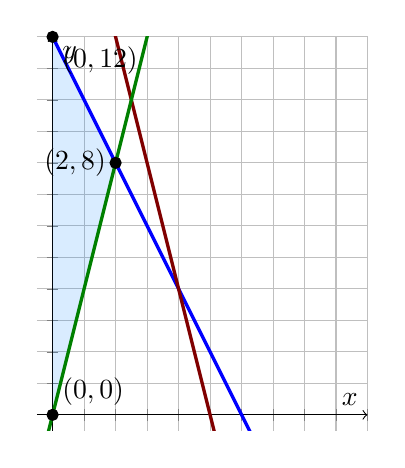
\begin{tikzpicture}
\begin{axis}[
    xmin=-0.5, xmax=10,
    ymin=-0.5, ymax=12,
    axis lines=center,
    axis on top=false,
    domain=0:1,
    x=0.4cm,
    y=0.4cm,
    xtick={0,1,...,10},
    xticklabels={},
    ytick={0,1,...,12},
    yticklabels={},
    axis lines=middle,
    axis line style={->},
    xlabel={$x$},
    ylabel={$y$},
    grid=major
    ]
    \addplot [thick,color=blue,fill=blue!50!cyan, 
                    fill opacity=0.15,draw opacity=0]coordinates {
            (0,0)
            (0,12)
            (2,8)  };
    \addplot [very thick,blue,domain=-10:10] {-2*x+12};
    \addplot [very thick,red!50!black,domain=-10:10] {-4*x+20};
    \addplot [very thick,green!50!black,domain=-10:10] {4*x};
	%\addplot [very thick,red!50!black] coordinates{(-3,-5)(-3,5)};
	
	\addplot [only marks,color=black] table {
	0 12
	0 0
	2 8
	};  
	\node[left] (A) at (axis cs:2,8) {$(2,8)$};
	\node[below right] (B) at (axis cs:0,12) {$(0,12)$};
	\node[above right] (D) at (axis cs:0,0) {$(0,0)$};
\end{axis}
\end{tikzpicture}
\end{center}
\end{itemize}\text{} \answer{$x=2$ magazine covers; $y=8$ logos; profit $=$ \$5600}

\item A manufacturer of ski clothing makes ski pants and ski jackets.  The profit on a pair of ski pants is \$2.00 and the profit on a jacket is \$1.50.  Both pants and jackets require the work of sewing operators and cutters.  There are 60 minutes of sewing operator time and 48 minutes of cutter time available.  It takes 8 minutes to sew one pair of ski pants and 4 minutes to sew one jacket.  Cutters take 4 minutes on pants and 8 minutes on a jacket.  Find the maximum profit and the number of pants and jackets the manufacturer should make in order to maximize the profit.
\begin{itemize}
\item Variables: $x=$ number of ski pants; $y=$ number of ski jackets
\item Objective function: $f = 2x + 1.5y$
\item Constraints: (plus $x \geq 0$ and $y \geq 0$)
\begin{align*}
8x + 4y &\leq 60\\
4x + 8y &\leq 48
\end{align*}

\item Feasible region and corner points:
\begin{center}
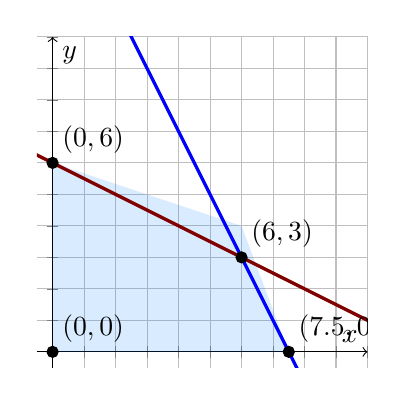
\begin{tikzpicture}
\begin{axis}[
    xmin=-0.5, xmax=10,
    ymin=-0.5, ymax=10,
    axis lines=center,
    axis on top=false,
    domain=0:1,
    x=0.4cm,
    y=0.4cm,
    xtick={0,1,...,10},
    xticklabels={},
    ytick={0,1,...,10},
    yticklabels={},
    axis lines=middle,
    axis line style={->},
    xlabel={$x$},
    ylabel={$y$},
    grid=major
    ]
    \addplot [thick,color=blue,fill=blue!50!cyan, 
                    fill opacity=0.15,draw opacity=0]coordinates {
            (0,0)
            (0,6)
            (6,4)
            (7.5,0)  };
    \addplot [very thick,blue,domain=-10:10] {-2*x+15};
    \addplot [very thick,red!50!black,domain=-10:10] {-0.5*x+6};
	%\addplot [very thick,red!50!black] coordinates{(-3,-5)(-3,5)};
	
	\addplot [only marks,color=black] table {
	0 6
	0 0
	6 3
	7.5 0
	};  
	\node[above right] (A) at (axis cs:6,3) {$(6,3)$};
	\node[above right] (B) at (axis cs:0,6) {$(0,6)$};
	\node[above right] (C) at (axis cs:7.5,0) {$(7.5,0)$};
	\node[above right] (D) at (axis cs:0,0) {$(0,0)$};
\end{axis}
\end{tikzpicture}
\end{center}
\end{itemize}\text{} \answer{$x=6$ ski pants; $y=3$ ski jackets; profit $=$ \$16.50}

\item An automotive plant makes the Quartz and the Pacer.  The plant has a maximum production capacity of 1200 cars per week, and they can make at most 600 Quartz cars and 800 Pacers each week.  If the profit on a Quartz is \$500 and the profit on a Pacer is \$800, find how many of each type of car the plant should produce.  What is the maximum profit?
\begin{itemize}
\item Variables: $x=$ number of Quartzes; $y=$ number of Pacers
\item Objective function: $f = 500x + 800y$
\item Constraints: (plus $x \geq 0$ and $y \geq 0$)
\begin{align*}
x + y &\leq 1200\\
x &\leq 600\\
y &\leq 800
\end{align*}

\item Feasible region and corner points:
\begin{center}
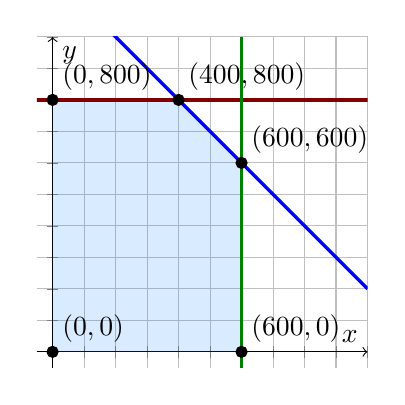
\begin{tikzpicture}
\begin{axis}[
    xmin=-0.5, xmax=10,
    ymin=-0.5, ymax=10,
    axis lines=center,
    axis on top=false,
    domain=0:1,
    x=0.4cm,
    y=0.4cm,
    xtick={0,1,...,10},
    xticklabels={},
    ytick={0,1,...,10},
    yticklabels={},
    axis lines=middle,
    axis line style={->},
    xlabel={$x$},
    ylabel={$y$},
    grid=major
    ]
    \addplot [thick,color=blue,fill=blue!50!cyan, 
                    fill opacity=0.15,draw opacity=0]coordinates {
            (0,0)
            (0,8)
            (4,8)
            (6,6)
            (6,0)  };
    \addplot [very thick,blue,domain=-10:10] {-x+12};
	\addplot [very thick,red!50!black] coordinates{(-1,8)(10,8)};
	\addplot [very thick,green!50!black] coordinates{(6,-1)(6,10)};
	
	\addplot [only marks,color=black] table {
	0 8
	0 0
	6 0
	6 6
	4 8
	};  
	\node[above right] (A) at (axis cs:4,8) {$(400,800)$};
	\node[above right] (B) at (axis cs:0,8) {$(0,800)$};
	\node[above right] (C) at (axis cs:6,6) {$(600,600)$};
	\node[above right] (D) at (axis cs:0,0) {$(0,0)$};
	\node[above right] (E) at (axis cs:6,0) {$(600,0)$};
\end{axis}
\end{tikzpicture}
\end{center}
\end{itemize}\text{} \answer{$x=400$ Quartzes; $y=800$ Pacers; profit $=$ \$840,000}

\item A farmer has a field of 70 acres in which he plants potatoes and corn.  The seed for potatoes costs \$20/acre, the seed for corn costs \$60/acre, and the farmer has set aside \$3000 to spend on seed.  The profit per acre of potatoes is \$150 and the profit for corn is \$50 an acre.  How many acres of each should the farmer plant?  What is the maximum profit?
\begin{itemize}
\item Variables: $x=$ acres of potatoes; $y=$ acres of corn
\item Objective function: $f = 150x + 50y$
\item Constraints: (plus $x \geq 0$ and $y \geq 0$)
\begin{align*}
x + y &\leq 70\\
20x + 60y &\leq 3000
\end{align*}

\item Feasible region and corner points:
\begin{center}
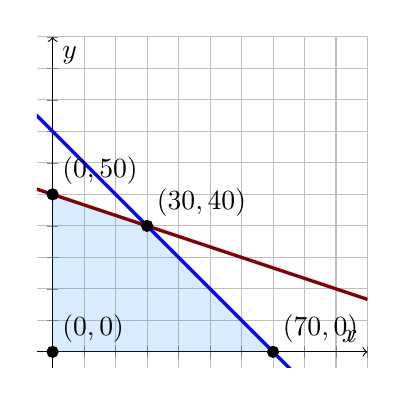
\begin{tikzpicture}
\begin{axis}[
    xmin=-0.5, xmax=10,
    ymin=-0.5, ymax=10,
    axis lines=center,
    axis on top=false,
    domain=0:1,
    x=0.4cm,
    y=0.4cm,
    xtick={0,1,...,10},
    xticklabels={},
    ytick={0,1,...,10},
    yticklabels={},
    axis lines=middle,
    axis line style={->},
    xlabel={$x$},
    ylabel={$y$},
    grid=major
    ]
    \addplot [thick,color=blue,fill=blue!50!cyan, 
                    fill opacity=0.15,draw opacity=0]coordinates {
            (0,0)
            (0,5)
            (3,4)
            (7,0)  };
    \addplot [very thick,blue,domain=-10:10] {-x+7};
    \addplot [very thick,red!50!black,domain=-10:10] {-x/3+5};
	
	\addplot [only marks,color=black] table {
	0 5
	0 0
	7 0
	3 4
	};  
	\node[above right] (A) at (axis cs:3,4) {$(30,40)$};
	\node[above right] (B) at (axis cs:0,5) {$(0,50)$};
	\node[above right] (C) at (axis cs:0,0) {$(0,0)$};
	\node[above right] (D) at (axis cs:7,0) {$(70,0)$};
\end{axis}
\end{tikzpicture}
\end{center}
\end{itemize}\text{} \answer{$x=70$ acres of potatoes; $y=0$ acres of corn; profit $=$ \$10,500}


\item A manufacturer produces two models of mountain bikes.  The times (in hours) required for assembling and painting each model are given by the following table:
\begin{center}
\begin{tabular}{|l|c|c|}
\hline
& Model A & Model B\\
\hline
Assembling & 5 & 4\\
\hline
Painting & 2 & 3\\
\hline
\end{tabular}
\end{center}
The maximum total weekly hours available in the assembly department and the painting department are 200 hours and 108 hours, respectively.  The profits per unit are \$25 for Model A and \$15 for Model B.  How many of each type should be produced to maximize profit?  What is the maximum profit?
\begin{itemize}
\item Variables: $x=$ number of Model A; $y=$ number of Model B
\item Objective function: $f = 25x + 15y$
\item Constraints: (plus $x \geq 0$ and $y \geq 0$)
\begin{align*}
5x + 4y &\leq 200\\
2x + 3y &\leq 108
\end{align*}

\item Feasible region and corner points:
\begin{center}
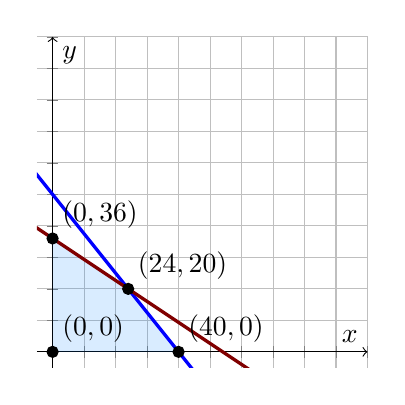
\begin{tikzpicture}
\begin{axis}[
    xmin=-0.5, xmax=10,
    ymin=-0.5, ymax=10,
    axis lines=center,
    axis on top=false,
    domain=0:1,
    x=0.4cm,
    y=0.4cm,
    xtick={0,1,...,10},
    xticklabels={},
    ytick={0,1,...,10},
    yticklabels={},
    axis lines=middle,
    axis line style={->},
    xlabel={$x$},
    ylabel={$y$},
    grid=major
    ]
    \addplot [thick,color=blue,fill=blue!50!cyan, 
                    fill opacity=0.15,draw opacity=0]coordinates {
            (0,0)
            (0,3.6)
            (2.4,2)
            (4,0)  };
    \addplot [very thick,blue,domain=-10:10] {-5*x/4+5};
    \addplot [very thick,red!50!black,domain=-10:10] {-2*x/3+3.6};
	
	\addplot [only marks,color=black] table {
	0 3.6
	0 0
	4 0
	2.4 2
	};  
	\node[above right] (A) at (axis cs:2.4,2) {$(24,20)$};
	\node[above right] (B) at (axis cs:0,3.6) {$(0,36)$};
	\node[above right] (C) at (axis cs:0,0) {$(0,0)$};
	\node[above right] (D) at (axis cs:4,0) {$(40,0)$};
\end{axis}
\end{tikzpicture}
\end{center}
\end{itemize}\text{} \answer{$x=40$ bikes of Model A; $y=0$ bikes of Model B; profit $=$ \$1000}
\pagebreak

\item A student earns \$10 per hour for tutoring and \$7 per hour as a teacher's aide.  To have enough free time for studies, he can work no more than 20 hours per week.  The tutoring center requires that each tutor spends at least three hours per week tutoring, but no more than eight hours per week.  How many hours should he work to maximize his earnings?  What are the maximum earnings?
\begin{itemize}
\item Variables: $x=$ hours tutoring; $y=$ hours as TA
\item Objective function: $f = 10x + 7y$
\item Constraints: (plus $x \geq 0$ and $y \geq 0$)
\begin{align*}
x + y &\leq 20\\
x &\geq 3\\
x &\leq 8
\end{align*}

\item Feasible region and corner points:
\begin{center}
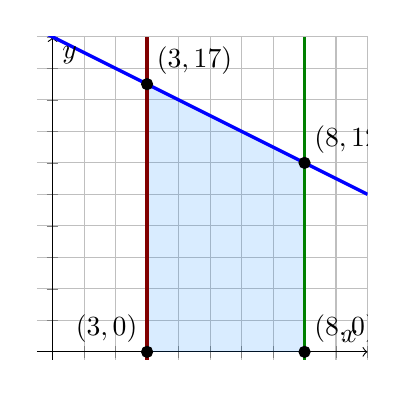
\begin{tikzpicture}
\begin{axis}[
    xmin=-0.5, xmax=10,
    ymin=-0.5, ymax=20,
    axis lines=center,
    axis on top=false,
    domain=0:1,
    x=0.4cm,
    y=0.2cm,
    xtick={0,1,...,10},
    xticklabels={},
    ytick={0,2,...,20},
    yticklabels={},
    axis lines=middle,
    axis line style={->},
    xlabel={$x$},
    ylabel={$y$},
    grid=major
    ]
    \addplot [thick,color=blue,fill=blue!50!cyan, 
                    fill opacity=0.15,draw opacity=0]coordinates {
            (3,0)
            (3,17)
            (8,12)
            (8,0)  };
    \addplot [very thick,blue,domain=-10:10] {-x+20};
	\addplot [very thick,red!50!black] coordinates{(3,-1)(3,20)};
	\addplot [very thick,green!50!black] coordinates{(8,-1)(8,20)};
	
	\addplot [only marks,color=black] table {
	3 0
	3 17
	8 12
	8 0
	};  
	\node[above left] (A) at (axis cs:3,0) {$(3,0)$};
	\node[above right] (B) at (axis cs:3,17) {$(3,17)$};
	\node[above right] (C) at (axis cs:8,12) {$(8,12)$};
	\node[above right] (D) at (axis cs:8,0) {$(8,0)$};
\end{axis}
\end{tikzpicture}
\end{center}
\end{itemize}\text{} \answer{$x=8$ hours tutoring; $y=12$ hours as a TA; profit $=$ \$164}
\end{enumerate}